\subsection{期刊投稿对\TeX 的需求}[\TeX in Academic Writing]\label{sec:jounaldemands}

\ppt{\TeX 与Word:地位变迁}
自1977年诞生以来,\TeX 及衍生的 \LaTeX, pdf\LaTeX, \XeLaTeX 等便因其高效高质的断行能力、数学式化学式支持、参考文献支持等优良特性迅速赢得出版业与学术界的用户的心。到了20世纪90年代,微软的Office Word终于具有了一定实力,从\TeX 阵营中分流了大部分仅有桌面出版需求的用户,但在学术界,\TeX 的强大功能及传统地位仍然难以撼动。

\ppt{\TeX:学术界地位}
当今,\TeX 与 Word 并行于当代国际主流学术界,几乎所有的学术机构都同时为两者提供支持。然而,在少数常见冗长而复杂的公式的数学、物理领域期刊,仅\TeX 能够满足为公式排版的苛刻技术要求,类似的场景在文献学期刊、计算机学期刊中屡见不鲜。

根据广泛参考,我们采用了学术界知名度最高的11个学术出报社(《自然》、《科学》、Springer、剑桥大学出版社、牛津大学出版社等)作为样本,考察其对\TeX 的支持情况。这些出版社在学术界享有标杆地位,是学术界出版的主流力量。

\begin{table}[!htb]
\caption{顶级学术期刊出版社\TeX 支持情况}
\label{pub}
\centering
\begin{tabular}{lcc}
\toprule
\ccell{出版社}&\ccell{\TeX 支持}&\ccell{\hskip5mm 提供模板文件}\\
\midrule
Nature Publishing Group&\ding{52}&\\
Science | AAAS	&\ding{52}&\ding{52}\\
Cambridge University Press&\ding{52}&\ding{52}\\
John's Hopkins University Press&\ding{52}&\\	
The MIT Press&\ding{52}&\ding{52}\\
Oxford University Press &\ding{52}&\ding{52}\\
Princeton University Press &\ding{52}&\ding{52}\\
University of Chicago Press &\ding{52}&\\
American Chemical Society (ACS)&\ding{52}&\ding{52}\\
Springer&\ding{52}&\ding{52}\\
Elsevier&\ding{52}&\ding{52}\\
\bottomrule
\end{tabular}
\end{table}

\begin{figure}[!htb]
\centering
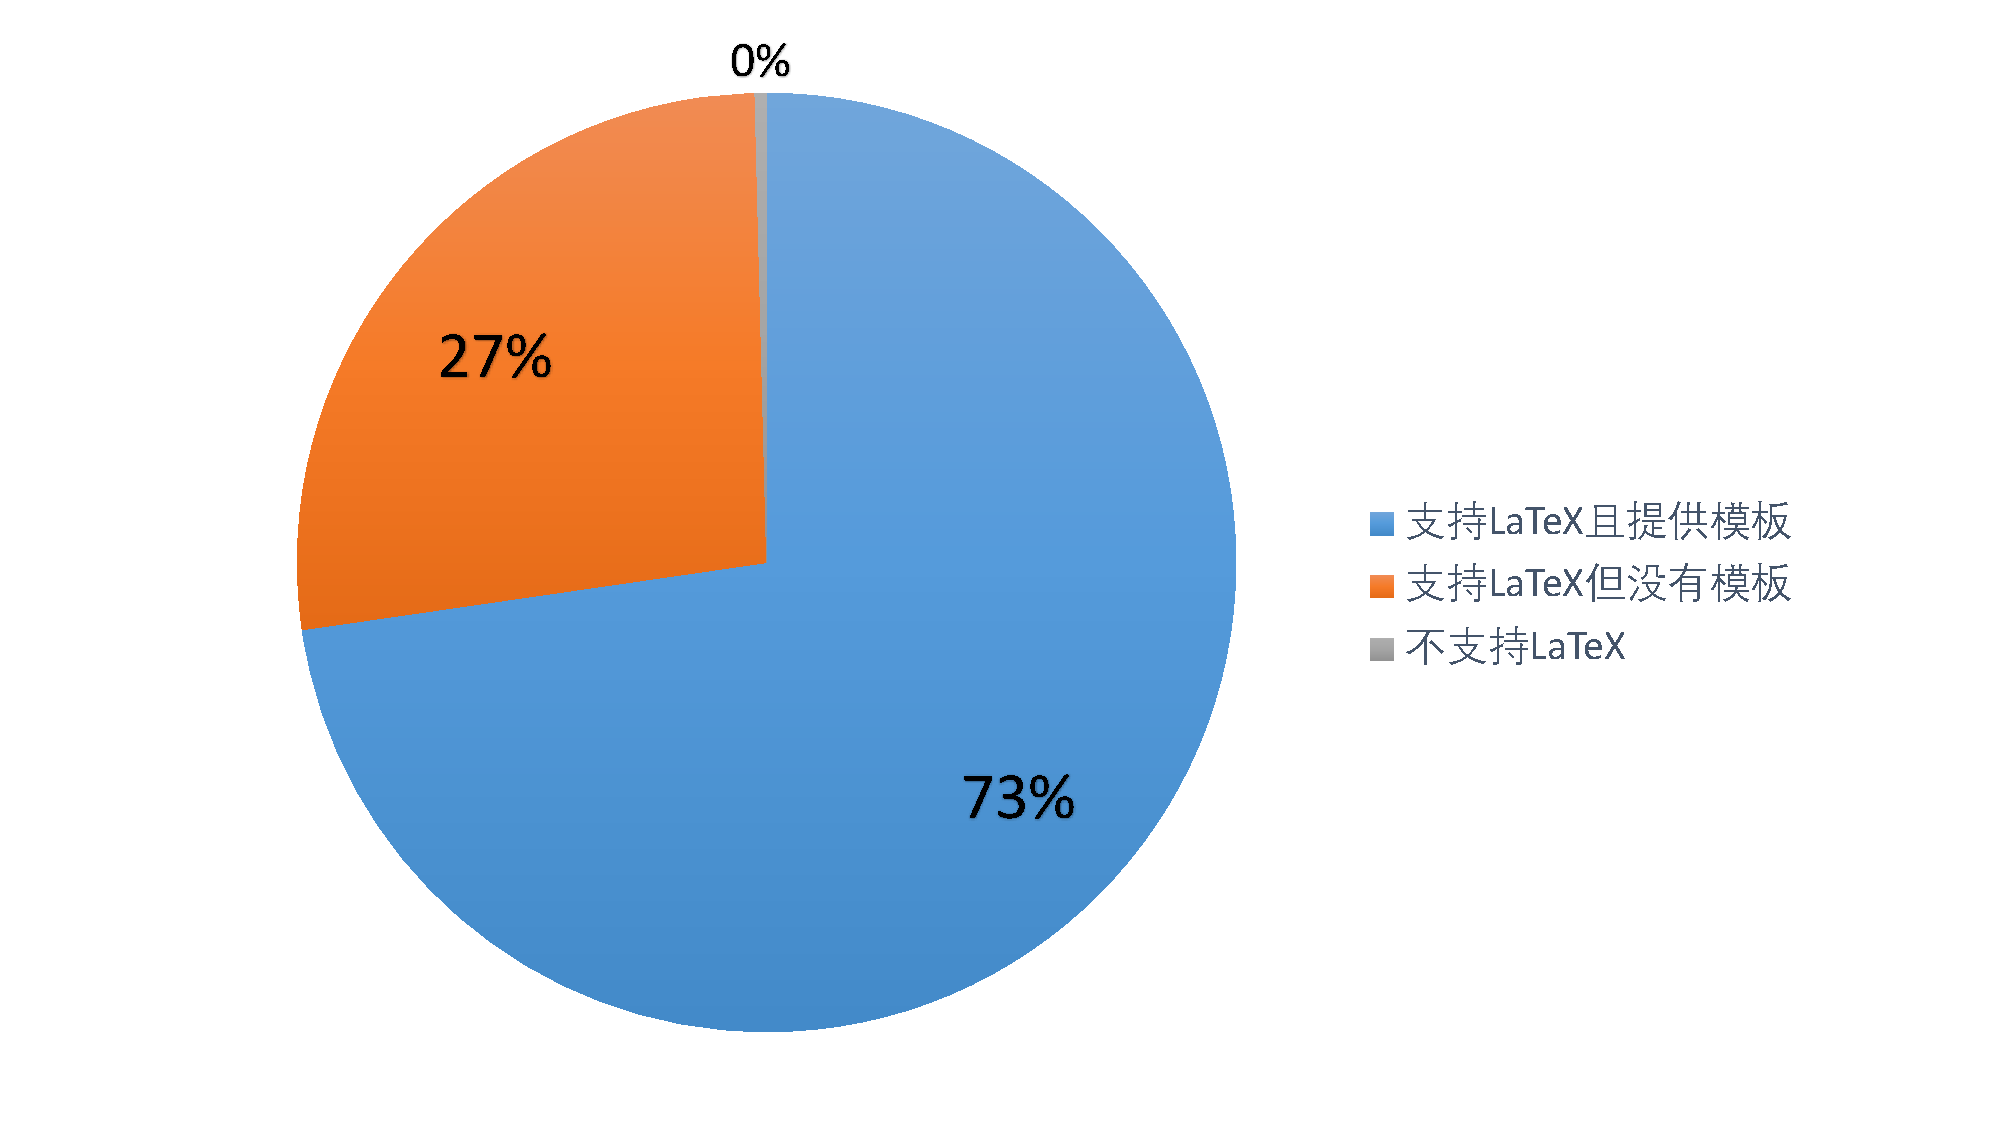
\includegraphics[width=\textwidth]{pubfig0}
\caption{顶级学术期刊出版社\TeX 支持情况}
\label{pubfig}
\end{figure}


调查显示样本库中所有顶级学术出版社均对使用\TeX 排版撰写的文章提供技术支持,其中73\%的学术出版社为作者提供\TeX 模板文件,极大便利了 \TeX 用户写作。(表\ref{pub}、图\ref{pubfig})
通过使用出版社提供的\TeX 模板文件,作者可以便利地排版出符合出版社格式要求和规范的论文,节约大量不必要的排版时间。

\ppt{\TeX:学术写作优势举例}
举个例子,在科研论文发表过程中,我们不可避免地会遇到学术文章需要由一部杂志改投其他杂志的情况,但是不同期刊的排版要求往往相差很大,从格式到文献引用方式可能都有不同,一点点修改调校则十分费时费力。好在,使用\TeX 来写作的论文可以直接改动文章排版时所依据的模板,这使得相同的文章在不同排版格式之间的便捷切换成为易事,这对提升研究人员投稿效率来说大有裨益。